\chapter{استنتاج نمودار کلاس طراحی}
در این مرحله، با استفاده از نمودار‌های توالی ایجاد شده در فصل قبل و همچنین گام‌ها و مراحل گفته شده در کتاب مرجع، کلاس‌ها، متد‌ها و صفت‌های کلاس‌ها شناسایی شدند. همچنین از مدل دامنه استفاده شد تا کلاس‌های اصلی برنامه را استخراج کنیم و نمودار‌‌های کلاس‌ها را تکمیل کنیم. در نهایت به کمک کلاس‌ها که بر اساس سبک معماری انتخابی به چهار بسته‌ی 
\lr{Front-end}،
\lr{Back-end}،
\lr{Data} و 
\lr{Network} 
تقسیم شده بودند و به طراحی و آماده‌سازی نمودار کلاس طراحی پرداخته شد.

\section{بسته‌ی \frontend}
این بسته مسئولیت نمایش صفحات مختلف، منو‌ها و دکمه‌های عملیاتی به کاربر را بر عهده دارد. صفحاتی مثل ...

\section{بسته‌ی \lr{Back-end}}
این بسته که مسئول پردازش تراکنش‌ها کسب و کار است، شامل در زیربخش به نام‌های \lr{business}  و \lr{controller} می‌باشد.

زیر بسته‌ی \lr{controller} شامل اشیا کنترل‌گر است که مسئول برخورد با رویداد‌های مربوط به یک یا چند مورد کاربرد هستند. 

در بسته‌ی کسب‌وکار،‌ کلاس‌های مربوط به کسب‌وکار که با کمک مدل دامنه و مورد کاربرد شناسایی شده بودند، قرار دارند.
\section{بسته‌ی \lr{Data}}
این بسته شامل شئ یا اشیا‌‌ئی‌ست که کار‌های مربوط به پابگاه داده که \lr{CRUD}\RTLfootnote{\lr{Create, Read, Update, Delete}} هستند را انجام می‌دهند 
\section{بسته‌ی \lr{Network}}
این بسته عملیات مربوط به ارتباطات سیستم به شبکه‌ی اصلی آن و شبکه‌ی اینترنت را فراهم می‌کند و بستر‌های لازم ارتباطی را فراهم می‌آورد.
\section{نمودار نهایی کلاس طراحی}
این نمودار در شکل \ref{pic:cd} آورده شده است.
\begin{figure}
	\begin{center}
		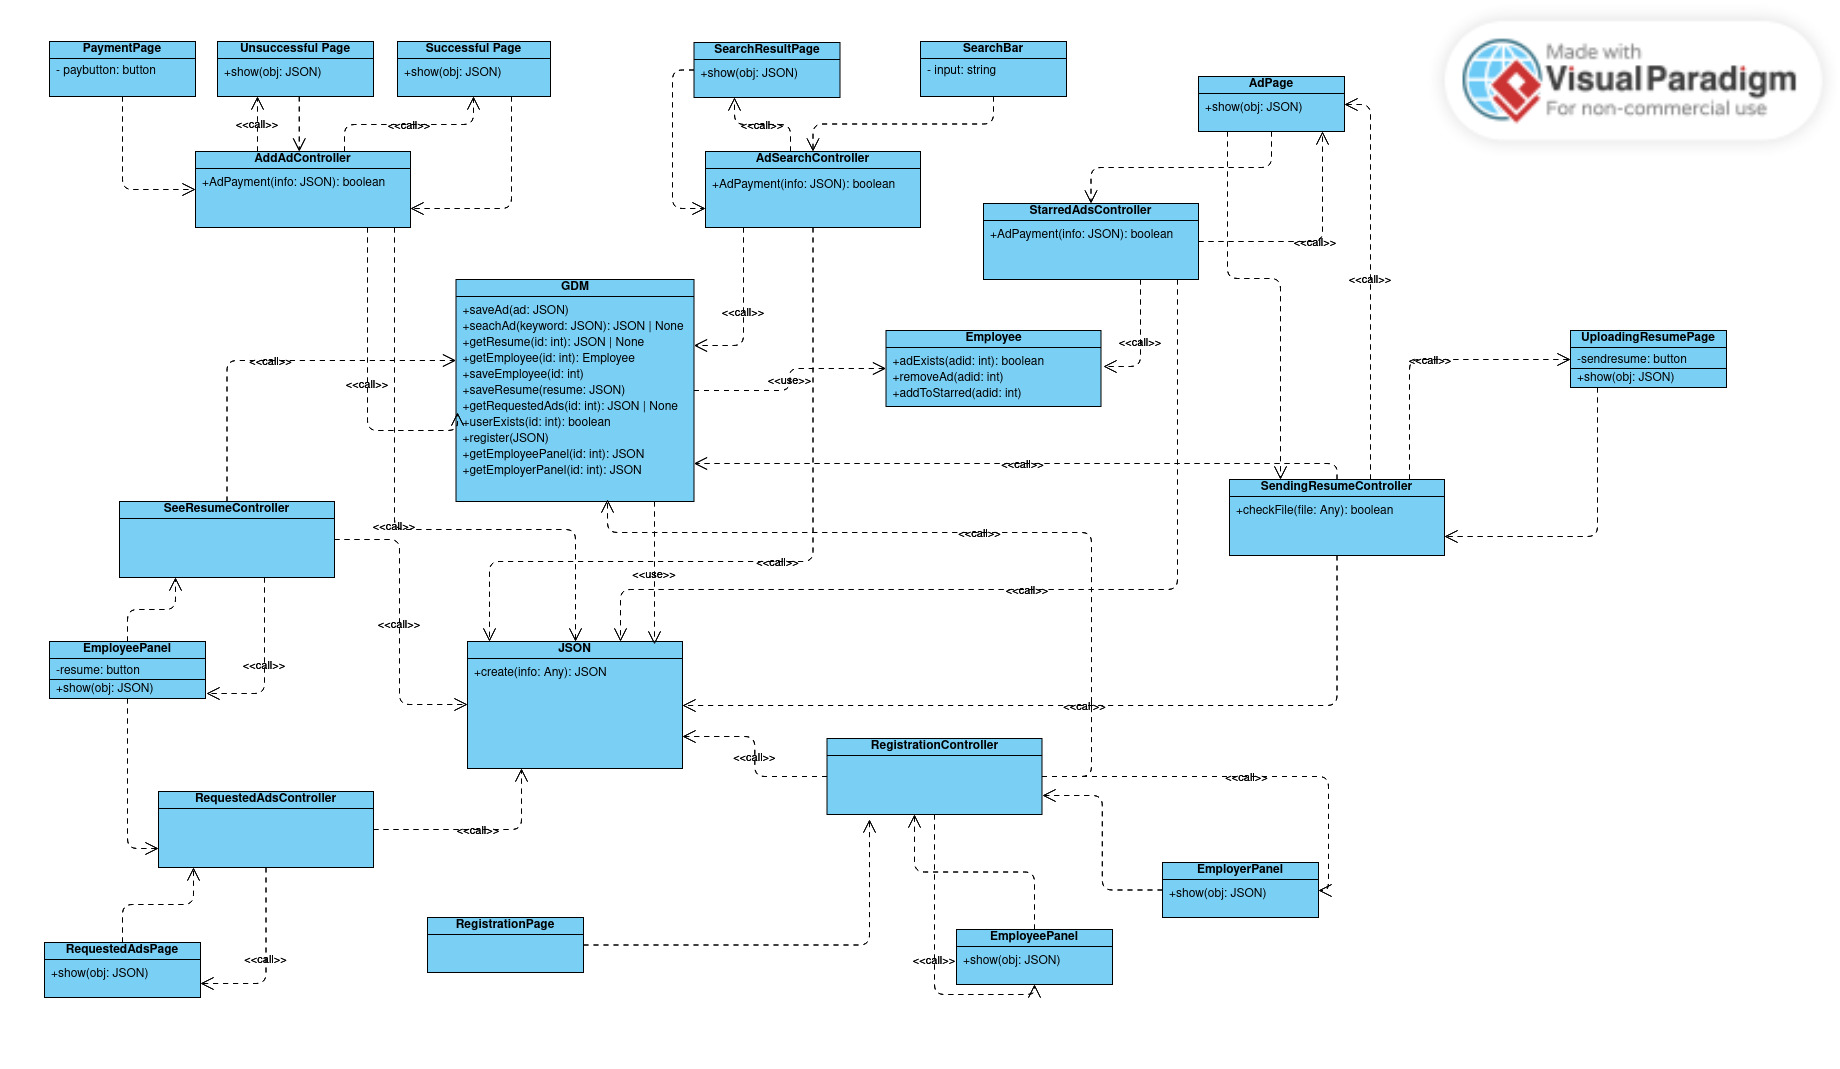
\includegraphics[width=\textwidth, angle=90, height=\textheight]{./images/cd}
	\end{center}
\caption{نمودار کلاس طراحی}
\label{pic:cd}
\end{figure}